

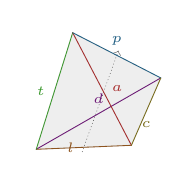
\begin{tikzpicture}[line join = round, line cap = round]

\coordinate (A) at (0.8737734,0.4020789,0.2735919); % incident to DPC (event node)
\coordinate (B) at (-0.5404401,0.6813372,-0.493664); % incident to TPA (step clocks!)
\coordinate (C) at (0.1666667,-0.787218,-0.5937256); % incident to LAC (origin anchor)
\coordinate (D) at (-0.5,-0.2961981,0.8137977); % incident to TLD (destination anchor)


% median lines: pick one
% \draw[->,color={rgb:red,1;green,1;blue,1}, densely dotted, line width = {0.2pt}] (A) -- (3*-0.2912578, 3*-0.1340263, 3*-0.0911973); % $TAL$ median
% \draw[->,color={rgb:red,1;green,1;blue,1}, densely dotted, line width = {0.2pt}] (B) -- (3*0.1801467, 3*-0.2271124, 3*0.1645547); % CDL median
% \draw[->,color={rgb:red,1;green,1;blue,1}, densely dotted, line width = {0.2pt}] (C) -- (3*-0.0555556, 3*0.262406, 3*0.1979085); % TPD median;
%\draw[->,color={rgb:red,1;green,1;blue,1}, densely dotted, line width = {0.2pt}] (D) -- (3*0.1666667, 3*0.0987327, 3*-0.2712659); % APC median;

% bimedian lines: pick one
 \draw[->,color={rgb:red,1;green,1;blue,1}, densely dotted, line width = {0.2pt}] (1.1*-0.16666665,1.1*-0.54170805,1.1*0.11003605) -- (1.1*0.16666665,1.1*0.54170805,1.1*-0.11003605); % $LP$ bimedian
% \draw[->,color={rgb:red,1;green,1;blue,1}, densely dotted, line width = {0.2pt}] (1.1*-0.1868867,1.1*-0.0529404,1.1*-0.5436948) -- (1.1*0.1868867,1.1*0.0529404,1.1*0.5436948); % $AD$ bimedian
% \draw[->,color={rgb:red,1;green,1;blue,1}, densely dotted, line width = {0.2pt}] (1.1*-0.52022005,1.1*0.19256955,1.1*0.16006685) -- (1.1*0.52022005,1.1*-0.19256955,1.1*-0.16006685); % $TC$ bimedian

% light shaded faces
\draw[-, fill={rgb:red,1;green,1;blue,1}, opacity=.05] (A)--(D)--(B)--cycle; % TDP
\draw[-, fill={rgb:red,1;green,1;blue,1}, opacity=.05] (A)--(D)--(C)--cycle; % CDL
\draw[-, fill={rgb:red,1;green,1;blue,1}, opacity=.05] (B)--(D)--(C)--cycle; % TAL
\draw[-, fill={rgb:red,1;green,1;blue,1}, opacity=.05] (A)--(B)--(C)--cycle; % APC

% color edges
\draw[-, color ={rgb:red,136;green,31;blue,147}, line width = {0.3pt}] (A)--(D); % D
\draw[-, color ={rgb:red,197;green,117;blue,43}, line width = {0.3pt}] (D)--(C); % L
\draw[-, color ={rgb:red,78;green,201;blue,59}, line width = {0.3pt}] (D)--(B); % T
\draw[-, color ={rgb:red,210;green,55;blue,55}, line width = {0.3pt}] (B)--(C); % A
\draw[-, color ={rgb:red,49;green,145;blue,201}, line width = {0.3pt}] (A)--(B); % P
\draw[-, color ={rgb:red,210;green,188;blue,45}, line width = {0.3pt}] (A)--(C); % C

% edge labels
\node[above, color={rgb:red,49;green,145;blue,201}] at (0.16666665,0.54170805,-0.11003605) {\tiny $p$}; % AB mean
\node[below, color={rgb:red,210;green,188;blue,45}] at (0.52022005,-0.19256955,-0.16006685) {\tiny$c$};  % AC mean
\node[above, color={rgb:red,136;green,31;blue,147}] at (0.1868867,0.0529404,0.5436948) {\tiny$d$};  % AD mean
\node[left, color={rgb:red,78;green,201;blue,59}] at (-0.52022005,0.19256955,0.16006685) {\tiny$t$};   % BD mean
\node[left, color={rgb:red,197;green,117;blue,43}] at (-0.16666665,-0.54170805,0.11003605) {\tiny$l$};  % CD mean
\node[right, color={rgb:red,210;green,55;blue,55}] at (-0.1868867,-0.0529404,-0.5436948) {\tiny$a$};  % BC mean

% node helper labels
%\node at (A) {\small A};
% \node at (B) {\small B};
% \node at (C) {\small C};
% \node at (D) {\small D};

\end{tikzpicture}

